% \documentclass[a4paper]{article}
\documentclass[twocolumn]{IEEEtran}

\usepackage[utf8]{inputenc}
\usepackage[T1]{fontenc}
\usepackage{graphicx}
\usepackage{hyperref}
\usepackage{amsmath}
\usepackage{amssymb}
\usepackage{amsthm}
\usepackage{mathenv}
\usepackage{multirow}
\usepackage{breqn}
\usepackage{rotating}


\DeclareMathAlphabet{\itbf}{OML}{cmm}{b}{it}

% numérotation au sein de chaque section (du style "2.1")
% \numberwithin{equation}{section}

% commandes perso
\newcommand{\R}{\mathbb{R}}
\newcommand{\ie}{i.e.}
\newcommand{\RnX}{\mathbb{R}_n[X]}
\newcommand{\N}{\mathbb{N}}
\newcommand{\C}{\mathcal{C}}
\newcommand{\Ccinf}{\mathcal{C}_c^{\infty}}
\newcommand{\Cinf}{\mathcal{C}^{\infty}}
\newcommand{\supp}{\textrm{supp}}
\newcommand{\bx}{\mathbf{x}}
\newcommand{\bv}{\mathbf{v}}
\newcommand{\Mbv}{M_{\mathbf{v}}}
\newcommand{\Tbv}{\mathcal{F}_{\mathbf{v}}}
\newcommand{\mubv}{\mu_{\mathbf{v}}}
\newcommand{\sbv}{s_{\mathbf{v}}}
\newcommand{\Bnv}{B_n^{(\bv)}}
\newcommand{\Wnv}{W_n^{(\bv)}}

\newtheorem{definition}{Definition}
\newtheorem{lemma}{Lemma}
\newtheorem{theorem}{Theorem}

\title{Consistency of Fan-beam Projections of a Translating Object Along an Arc of a Circle}
%\author{}
\date{}

\begin{document}

%==================
\author{
	\IEEEauthorblockN{Thomas Boulier, Rolf Clackdoyle, Jérôme Lesaint, Laurent Desbat}
	\thanks{T. Boulier, R. Clackdoyle, J. Lesaint and L. Desbat are with the TIMC-IMAG laboratory, CNRS UMR 5525 and Universit\'e Grenoble Alpes (e-mail: thomas.boulier@polytechnique.edu).

	The authors would like to thank Simon Rit for his help using RTK.
			
	This work is partially supported by the Agence Nationale de la Recherche (France), project ``DROITE'', number ANR-12-BS01-0018, and FUI project "3D4Carm".
}		
\IEEEauthorblockA{}
}

\maketitle
%========================

\begin{abstract}
In this article, we compute data consistency conditions (DCCs) in fan-beam geometry for the case of a translating object irradiated by an x-ray source moving along a short arc of a circle. The DCCs are thus a generalization of those computed in~\cite{clackdoyle2015consistency}, where the object remained still. In a second part, we use the DCCs in order to retrieve parameters of the object velocity. These results are illustrated by numerical examples.
\end{abstract}

\section{Introduction}

In the field of CT-imaging, data consistency conditions (DCCs) use the redundancy of the data in order to establish relations that must be fulfilled  between projections. These conditions are called \emph{full} when they are not only necessary but also sufficient. One of the best known DCCs are the Helgason-Ludwig (H-L) conditions~\cite{helgason1980radon,ludwig1966radon}, which are full for parallel projections. Full DCCs are also known for the case of fan-beam projections with source position taken along a straight line~\cite{clackdoyle2013necessary}.

In~\cite{clackdoyle2015consistency}, the fan-beam DCCs were modified to handle the case of a source moving along an arc of a circle. Briefly, all rays passing through the same point along a "virtual" source line between the two extreme positions of the source are gathered to form a virtual fan-beam projection. The DCCs for fan-beam projections along a line from~\cite{clackdoyle2013necessary} could then be applied; numerical examples showed a situation where an artificial detector attenuation was added, and the DCCs were invoked to recover the unknown attenuation coefficient. The case of a moving object has been tackled in~\cite{yu2006data,yu2007data}, where the authors used parallel-beam H-L conditions for the case of an object undergoing rigid body motion while irradiated by a fan-beam source along a circular trajectory. Those conditions allowed the authors to recover the parameters of the the movement. The parameters were subsequently incorporated into the reconstruction procedure, in order to suppress the artifacts caused by such movement.  However, using the parallel-beam H-L conditions means that the fan-beam projections had to cover all rays in the plane so that a fan-to-parallel rebinning could be achieved. The rebinning was achieved mathematically; however, the requirement of at least a standard fan-beam shortscan of $180^{\circ}$ plus fan-angle was required. In our work, we are concerned with the opposite extreme of a short arc of fan-beam measurements.

In this article, we will suppose that an object is translating while illuminated by a fan-beam source which is moving along an arc of a circle. Using a change of reference frame, we will use the same idea as in~\cite{clackdoyle2015consistency} a change of variables. Then, in a second part, we will show how the DCCs can be used in order to identify the translation velocity.

\section{Theory} 
\label{sec:theory}

\subsection{Problem under consideration}
\label{sub:problem_under_consideration}

Let us begin with some notation and definitions. We will consider an object in $\R^2$ to be imaged in a fan-beam geometry with sources on an arc of circle with center $O$ and radius $R_0$ (see Figure~\ref{fig:notations}, top). The object is identified with its density function $\mathbf{x} \mapsto \mu(\mathbf{x}) \in \Ccinf(\R^2)$.
\begin{figure}[!ht]
	\centering
	\begin{tabular}{c}
	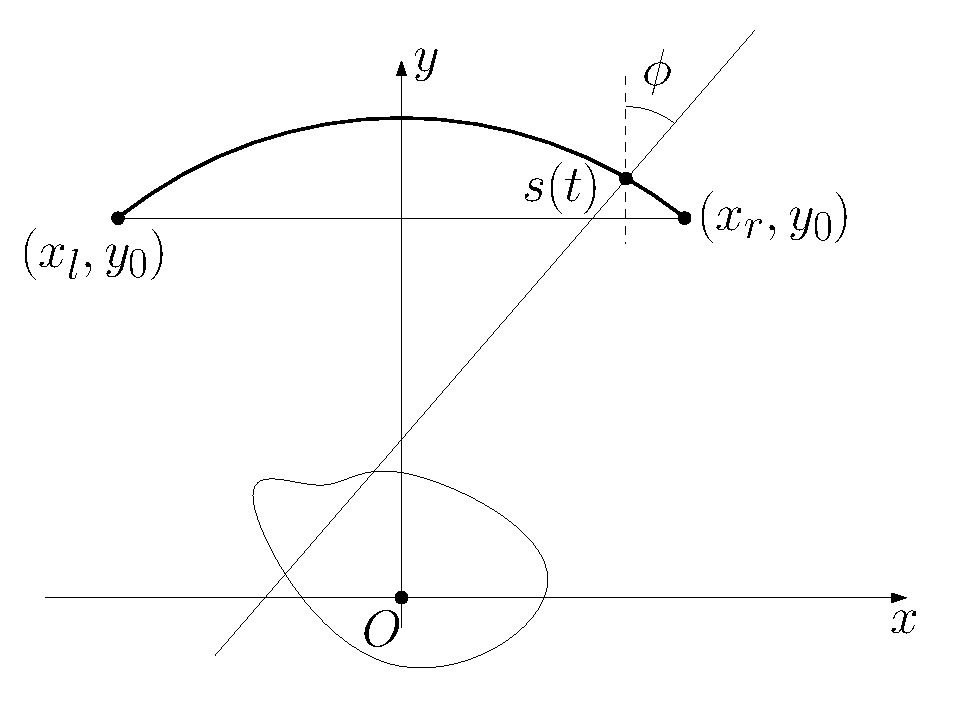
\includegraphics[width=60mm]{figs/frame_scanner_still.eps} \\
	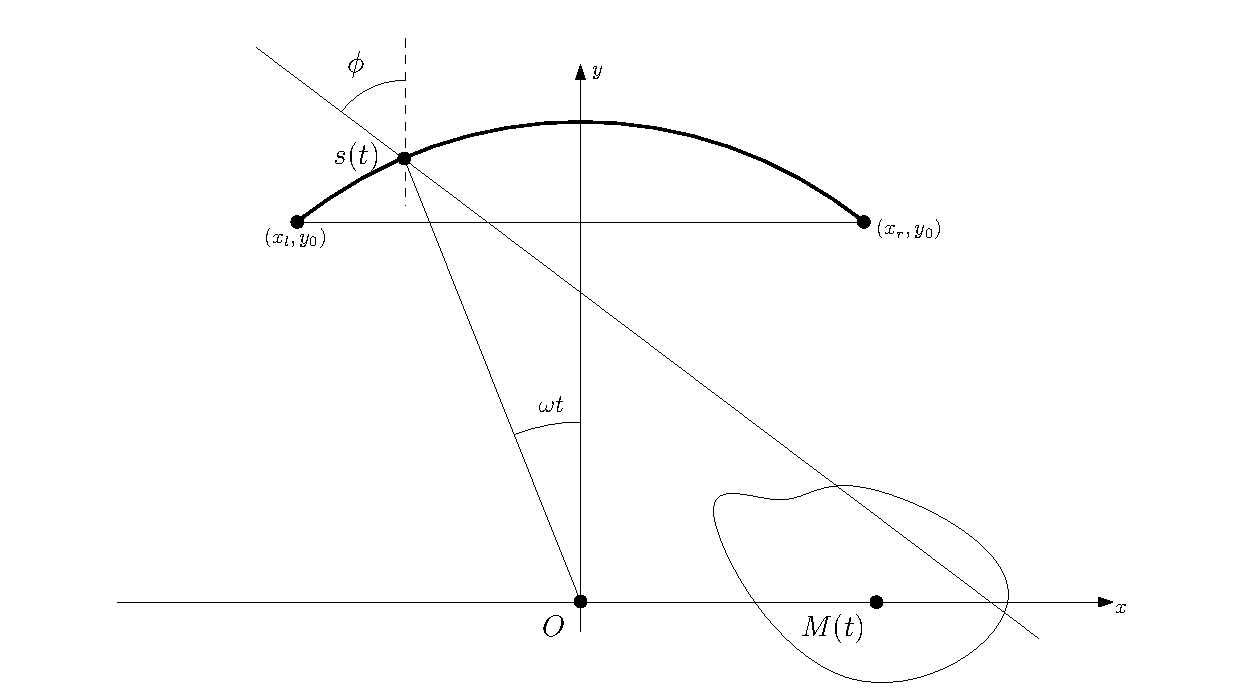
\includegraphics[width=60mm]{figs/frame_scanner.eps}
	\end{tabular}
	\caption{Problem under consideration. The source point $s(t)$ follows the arc of circle depicted in bold. The circle has center $O$ and radius $R_0$. The object is continually undergoing a translation during the movement of the source.\label{fig:notations}}
\end{figure}
The angular velocity of the source will be denoted $\omega$, and the time $t$ will range from $-T/2$ to $T/2$, where $T>0$. Hence, if we use $s(t)$ to denote the position of the source at time $t$, we have
\begin{equation}
	s(t) = \left( -R_0 \sin(\omega t), R_0 \cos(\omega t) \right).
\label{eq:source_position}
\end{equation}
Furthermore, we will let $s(T/2)=(x_l,y_l)$ (resp. $s(-T/2)=(x_r,y_r)$) denote the extreme left (resp. right) position of the source. Since $y_l = y_r = R_0 \cos(\omega T/2)$, we will call the common value $y_0$. In the following, we will assume that $\supp(\mu)$ lies in the half-space $\{ y < y_0 \}$, and that $y_0 > 0$ (\ie $0 < \omega T < \pi$, the total arc length is less than $\pi$).

We will suppose that at any time $t$, rays are simultaneously emitted from the source $s(t)$ with each ray at angle $\phi$ ranging from $-\pi/2$ to $\pi/2$. With this setup in mind, we can define the operator modeling the acquired data from the object.
\begin{definition}
The \emph{fan-beam projection data} of an object with density function $\mu$ is a function $(t,\phi) \mapsto \mathcal{F}\mu(t,\phi)$ defined by
\begin{equation}
	(\mathcal{F}\mu)(t,\phi) = \int_0^{+\infty} \mu \left( s(t) + l \left[ \sin \phi, -\cos \phi \right] \right) dl,
\end{equation}
where $t \in \left[ -T/2, T/2\right]$, $\phi \in \left[ -\pi/2, \pi/2\right]$ and $s(t)$ is given by~(\ref{eq:source_position}). The operator $\mu \mapsto \mathcal{F}\mu$ is called the \emph{fan-beam projection operator}.
\end{definition}


Now let us suppose that the object is translating along a straight line with a constant velocity vector $\bv = (v_1, v_2)\in \R^2$ (see Figure~\ref{fig:notations}, bottom). In other words, if we let $\Mbv(t)$ denote its center of mass at any time $t$, we have
\begin{equation}
	\Mbv(t) =   \left( t + T/2 \right) \bv
\label{eq:center_of_mass}
\end{equation}
The density function of the object now depends on both the spatial variable $\bx \in \R^2$ and the time $t$. If we denote the time-varying object by $\mubv$, we have
\begin{equation}
	\mubv(t,\bx) = \mu\left( \bx - \Mbv(t)\right).
\end{equation}
In this regard, the fan-beam projection data will be modified in the following way.
\begin{definition}
The \emph{fan-beam projection data of a translating object} with density function $\mu$ and  velocity vector $\bv$ is given by
\begin{equation}
	(\Tbv\mu)(t,\phi) =  ( \mathcal{F} \mubv ) (t,\phi).
\label{eq:def_Tv}
\end{equation}
\end{definition}

The aim of this note is to derive data consistency conditions (DCCs) from~(\ref{eq:def_Tv}), in order to retrieve the velocity vector $\bv$ from the knowledge of a single element of the range of $\Tbv$.

\subsection{Derivation of DCCs}

In order to derive DCCs, we will first change our reference frame, from $\left(O, x, y\right)$ to $\left(M(t), x', y'\right)$, so that the origin is the center of mass of the object at any time $t$, and the line between the start point and the end point of the source is still parallel to the $x'$-axis (see Figure~\ref{fig:change_frame}). In other words, we are performing the following change of variables
\begin{equation}
	(x,y) \leftrightarrow (x',y') = \mathcal{R}_{\beta} \left( (x,y)-\Mbv(t) \right),
\end{equation}
where $\mathcal{R}_{\beta}$ rotation by $\beta$. Note that the translation depends on $t$, but a single global rotation is applied. The angle $\beta$ is depicted in Figure~\ref{fig:change_frame} (top) and is given by
\begin{equation}
	\beta = \arctan \left( \frac{T v_2}{2R_0 \sin(\omega T/2) + T v_1} \right).
\end{equation}
Note that in this equation, the denominator can be equal to zero. This situation can occur in particular cases when $v_1 < 0$. We have studied those particular cases, both in terms of physical meaning and numerical implications. For the sake of simplicity, we will assume that $v_1$ is not too negative (e.g. $v_1 > - 2 R_0 / T$) to ensure that the denominator is non-zero.

\begin{figure}[!ht]
	\centering
	%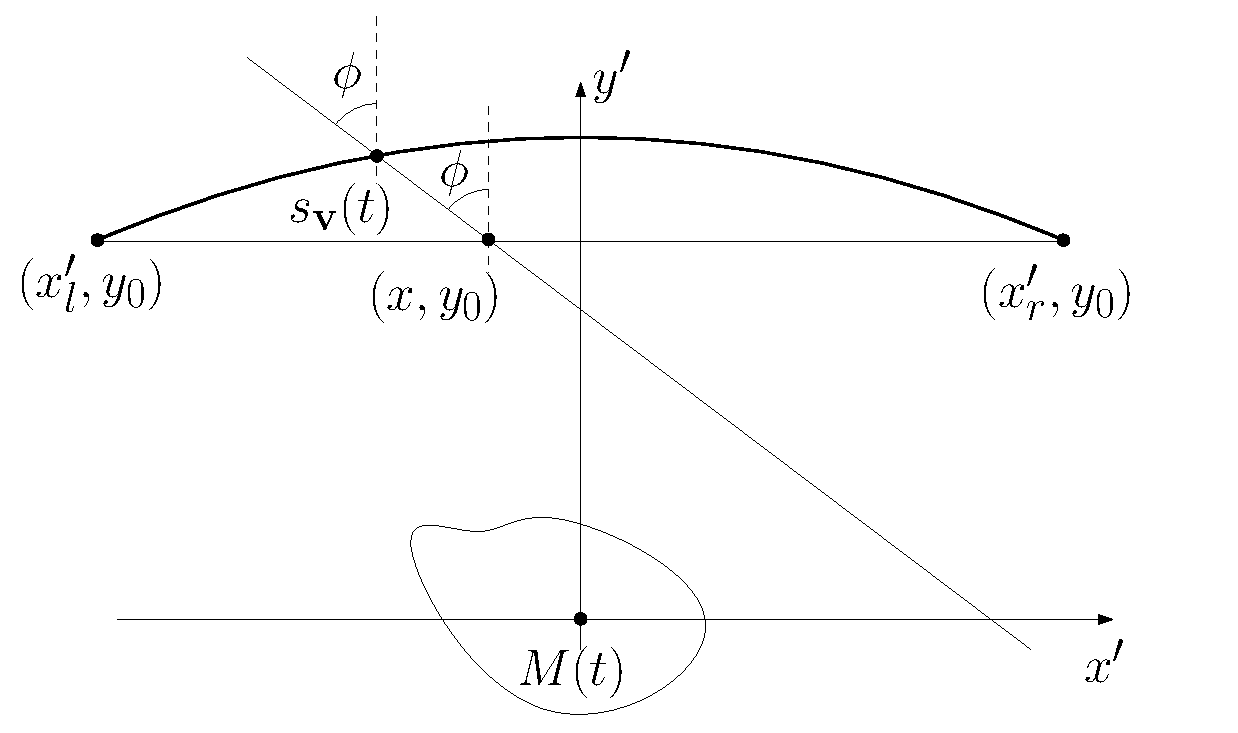
\includegraphics[width=12cm]{figs/frame_object.eps}
	\begin{tabular}{c}
	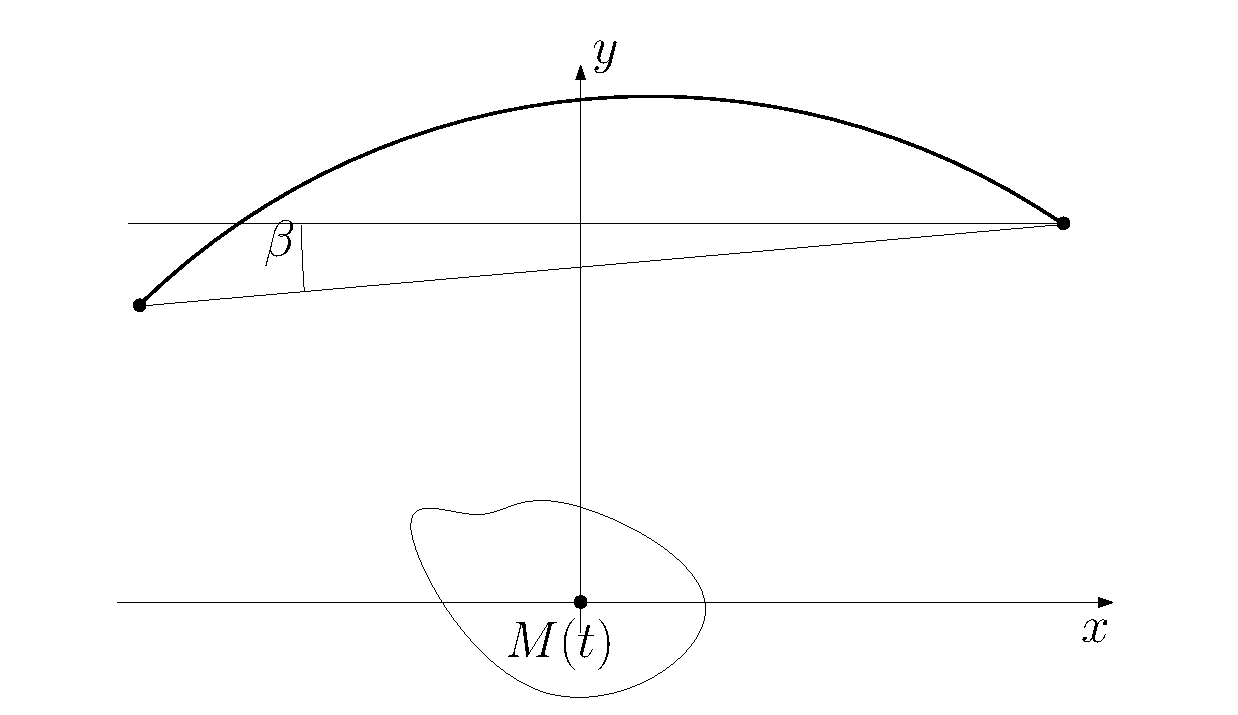
\includegraphics[width=70mm]{figs/frame_object_before_rotation.eps} \\
	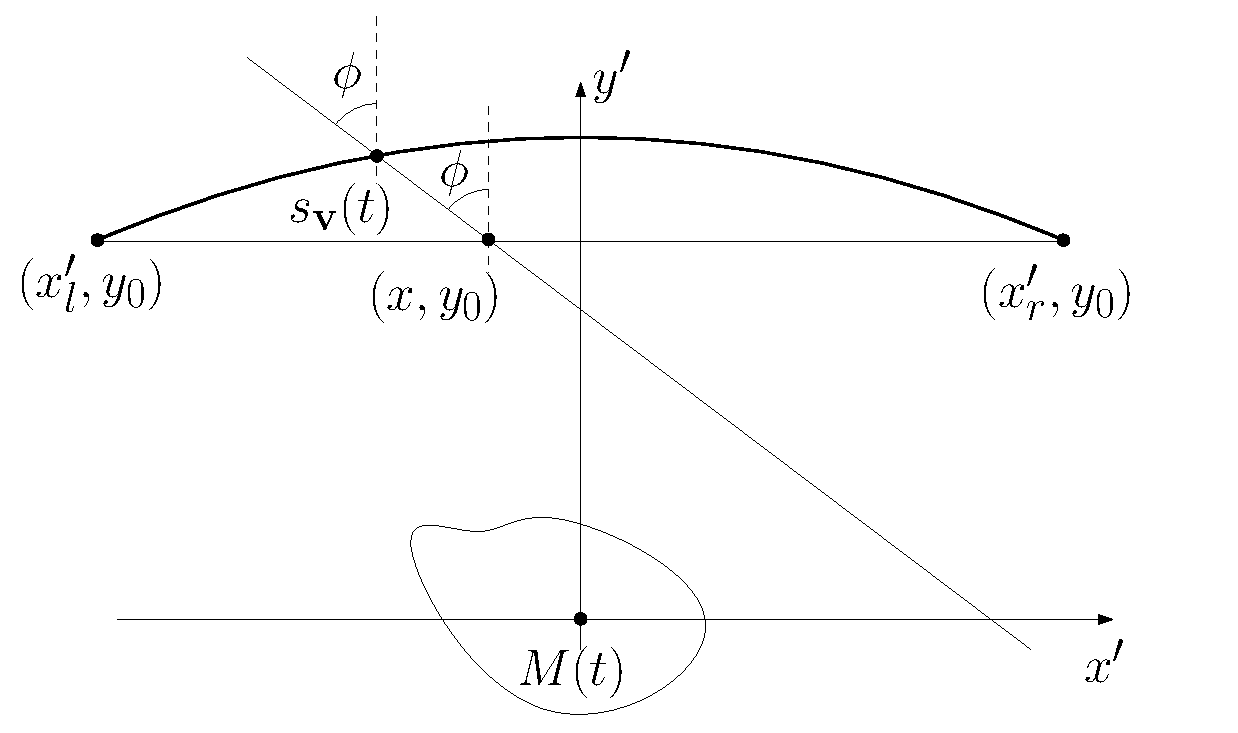
\includegraphics[width=70mm]{figs/frame_object.eps}
	\end{tabular}
	\caption{Change of reference frame: the object is now at center of the coordinate system. Top: only translation of the center of frame; bottom: after rotation of angle $\beta$. The virtual source position $(x',y_0')$ is defined in terms of $\sbv(t)$ and $\phi$; see equation~(\ref{eq:x'}).\label{fig:change_frame}}
\end{figure}

In this new reference frame, the coordinates of the source position are given by $\sbv(t)=\mathcal{R}_{\beta} \left( s(t)-\Mbv(t) \right)$. With this in mind, the data are given by the following formula
\begin{multline}
	(\Tbv\mu)(t,\phi) = \\
	\int_0^{+\infty} \mu \circ \mathcal{R}_{-\beta} \left( s_{\bv}(t) + l \left[ \sin (\phi + \beta), -\cos (\phi + \beta) \right] \right) dl,
\label{eq:F_from_sv}
\end{multline}

In other words, we are now dealing with a fixed object whose density function is given by $\mu \circ \mathcal{R}_{-\beta}$ irradiated by a source following an arc of a cycloid in the frame $\left(M(t), x', y'\right)$ (see Figure~\ref{fig:change_frame}, bottom).

Here, the extreme points $\sbv(-T/2)$ and $\sbv(T/2)$ have the same $y'$-coordinate, $y'_0$. We will call $x'_l$ (resp. $x'_r$) the $x'$-coordinates of $\sbv(T/2)$ (resp. $\sbv(-T/2)$).

Now we define what we call the \emph{virtual fan-beam projection} from a point $(x',y'_0)$.
\begin{definition}
	For any point $x'$ between $x'_l$ and $x'_r$, and for any angle $\phi \in \left[ -\pi/2, \pi/2\right]$, the \emph{virtual fan-beam projection} of the object $\mu$ is defined by
\begin{multline}
	\left( \tilde{\mathcal{F}} \mu	\right)(x',\phi') = \\
	\int_0^{+\infty} \mu \circ \mathcal{R}_{-\beta} \left( (x',y'_0) + l \left[ \sin \phi', -\cos \phi' \right] \right) dl.
\label{eq:def_Ftilde}
\end{multline}
This is called \emph{virtual} since it does not correspond to an actual position of the source.
\end{definition}

In the following lemma, we will make the connection between the virtual fan-beam projection and the fan-beam projection of the translating object.
\begin{lemma}
	Let us fix a time $t \in \left[ -T/2, T/2\right]$ and an angle $\phi \in \left[ -\pi/2, \pi/2\right]$. Let us define
	\begin{equation}
		x' = s_{1,\bv}(t) + \tan \phi \left( s_{2,\bv}(t) - y'_0 \right),
		\label{eq:x'}
	\end{equation}
	where, for any time $t$, $\left( s_{1,\bv}(t), s_{2,\bv}(t) \right)$ are the coordinates of $\sbv(t)$.
	Then, we have $\left( \tilde{\mathcal{F}} \left( \mu \circ \mathcal{R}_{-\beta} \right) \right)(x',\phi + \beta) = \left( \Tbv \mu \right)(t,\phi)$.
\label{lem:T_x_t}
\end{lemma}
The idea behind the proof of lemma~\ref{lem:T_x_t} is to note that between $x'$ and $\sbv(t)$, the integral of $\mu$ is equal to zero since the support is assumed to remain in the half-space $\left\{ y<y_0 \right\}$. Hence, instead of starting the integration from $x'$ in~(\ref{eq:def_Ftilde}), we can start from $\sbv(t)$, which will give us~(\ref{eq:F_from_sv}).

We can now define the DCCs for our problem.
\begin{theorem}
\label{theo:main}
Let us fix a density function $\mu$. For any integer $n$, there exists a function $(t,x')\mapsto \Wnv(t,x')$ such that the function $\Bnv$ defined by
\begin{equation}
	\Bnv(x') = \int_{-T/2}^{T/2} \left( \Tbv \mu \right)\left( t,\lambda^{(\bv)}(t,x') \right) \Wnv(t,x') dt,
\label{eq:DCC}
\end{equation}
is a polynomial of degree $n$. In the formula above, the angle $\lambda^{(\bv)}(t,x')$ is defined by
\begin{equation}
	\lambda^{(\bv)}(t,x') = \arctan \left( F^{(\bv)}(t,x') \right),
\label{eq:def_lambda}
\end{equation}
where $F^{(\bv)}(t,x')$ is defined as the fraction $A/B$ with
\begin{dmath}
	A = x' + \cos \beta \left( R_0 \sin(\omega t) + \left( t + T/2 \right)v_1 \right) + \\
	\sin \beta \left( R_0 \cos(\omega t) - \left( t + T/2 \right)v_2 \right)
\end{dmath}
and
\begin{dmath}
	B = \cos \beta \left( R_0 \cos(\omega t) - \left( t + T/2 \right)v_2 \right) - \sin \beta \left( R_0 \sin(\omega t) + \left( t + T/2 \right)v_1 \right) - y'_0 
\end{dmath}
Moreover, it is possible to derive $\Wnv(t,x')$ analytically using the following formula
\begin{multline}
	\Wnv(t,x') = \\
	\tan^n \left( \lambda^{(\bv)}(t,x') \right) \cos \left( \lambda^{(\bv)}(t,x') \right) \frac{\partial \lambda^{(\bv)}}{\partial t} (t,x')
\end{multline}
\end{theorem}

We only have room here for an outline of the proof. The idea is to change variables in the following formula, which is known from~\cite{clackdoyle2013necessary} to be a polynomial in $x'$
\begin{equation}
	\int_{\pi/2}^{-\pi/2} \tilde{\mathcal{F}}\mu (x',\phi) \frac{\tan^n \phi}{\cos \phi} d\phi.
\label{eq:DCC_rolf}
\end{equation}
The change of variable occurs between $\phi$ in~(\ref{eq:DCC_rolf}) and $t$ in~(\ref{eq:DCC}) by using the definition in~(\ref{eq:def_lambda}).

Although the formula for $\Wnv(t,x')$ is complicated, we observe that in the case $v_1=v_2=0$, we obtain the formula (7) in~\cite{clackdoyle2015consistency} since
\begin{equation}
	F^{\left( (0,0)\right) }(t,x')= \frac{x' + R_0 \sin(\omega t)}{R_0 \cos(\omega t)}
\end{equation}

\section{Numerical simulations}

\subsection{Principles}
\label{sub:principles}
Let us suppose that we have the projections $\left( \Tbv \mu \right)(t,\phi)$. Moreover, we suppose that $T$ is known and that the velocity $\bv$ is constant (although unknown) during the interval $[-T/2, T/2]$. In order to recover $\bv$, we can perform the following optimization procedure. Since $\Bnv(x')$ in equation~(\ref{eq:DCC}) is supposed to be a polynomial of degree less than or equal to $n$, we can minimize
\begin{equation}
	\mathcal{J}(v) = \Vert \left( \textrm{res} \Bnv \right) \Vert^2
\label{eq:Jv}
\end{equation}
with respect to $\bv$, where $\textrm{res}$ is the residual of the projection onto the space of polynomials of degree $n$ or less, and $n$ is the polynomial degree to be taken into account. This procedure will give us the velocity $\bv$ using only the knowledge of the data $\left( \Tbv \mu \right)(t,\phi)$.

\subsection{Application}
\label{sub:application}

The object under consideration is an ellipse of uniform density, whose axis lengths are $30$ and $15$ millimeters respectively, and making an angle of $45^{\circ}$ with respect to the $x$-axis. The source is rotating around the object with radius $R_0 = 600 \, \textrm{mm}$, with angular velocity $\omega = 1 \, \textrm{rad} \cdot \textrm{s}^{-1}$. The detector is a plane situated at a distance of $600 \, \textrm{mm}$ from the origin. The computations of the forward problem were performed using \verb+simpleRTK+, a Python wrapping of \verb+RTK+~\cite{RTK}.

With the simulated velocity of the ellipse given by $v_1 = 0.3 \, \textrm{mm} \cdot \textrm{s}^{-1}$, and $v_2 = 0 \, \textrm{mm} \cdot \textrm{s}^{-1}$ we obtain the sinogram depicted in Figure~\ref{fig:sinogram}.
\begin{figure}[!ht]
	\centering
	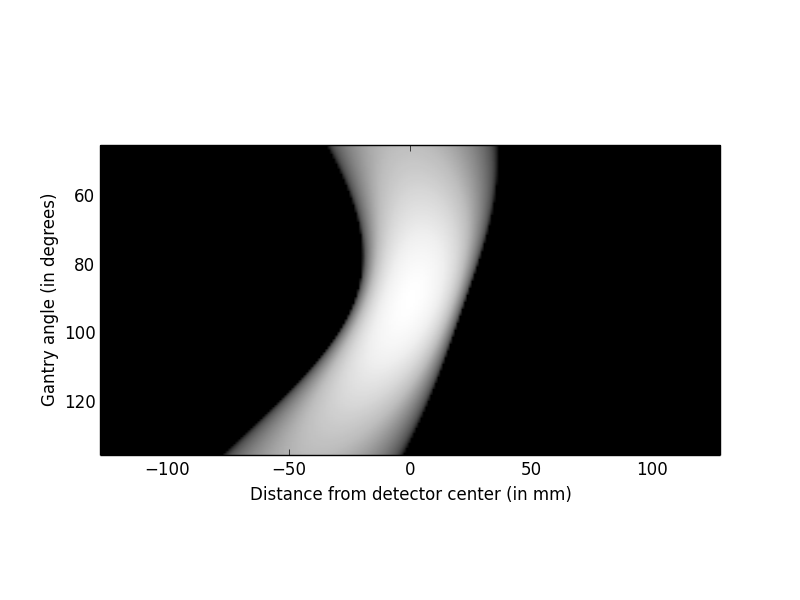
\includegraphics[width=70mm]{figs/sinogram.png}
	\caption{Sinogram of a moving ellipse, with semi-axis $a = 30$ and $b = 15$, translating along the $x$-axis with velocity $\bv = (0.3,0)$. It is irradiated by a source at distance $R_0 = 600$, rotating with angle velocity $\omega = 1$. Gantry angle represents the angular position of the source, with respect to the $x$-axis $(= \omega t + \pi/2)$; see Figure~\ref{fig:notations}. The object translation occurs between gantry angles $45^{\circ}$ and $90^{\circ}$.\label{fig:sinogram}}
\end{figure}

With this configuration in mind, the functions $x' \mapsto \Bnv(x')$ for $n = 0,1,2,3$ were calculated from the simulated sinogram, and are illustrated in Figure~\ref{fig:Bnx}. Note that these expressions for $\Bnv$, follow the predicted pattern of $n^{\textrm{th}}$-degree polynomials, as can be seen by the fact that root mean square errors (RMSEs) between the actual values of $\Bnv(x)$ and their best polynomial approximations are low.
\begin{figure}
	\centering
	\begin{tabular}{cc}
	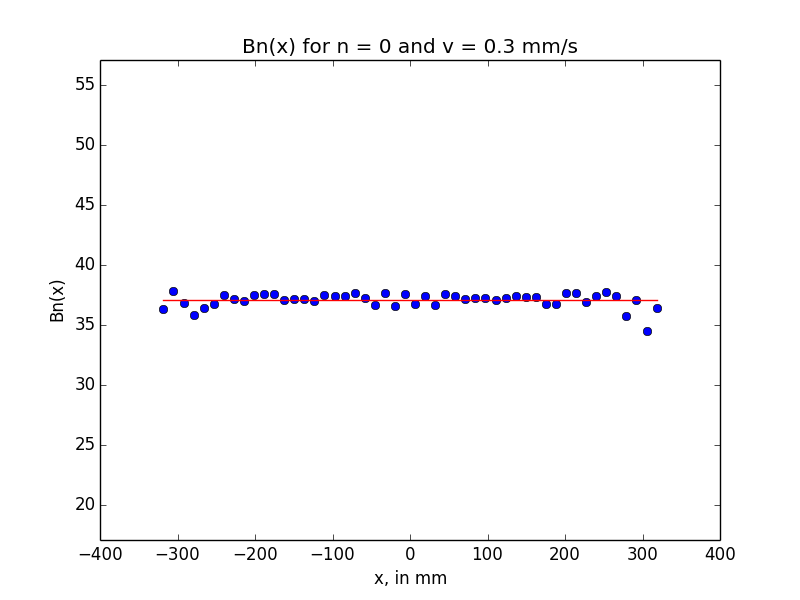
\includegraphics[width=75mm]{figs/B0.png} \\
	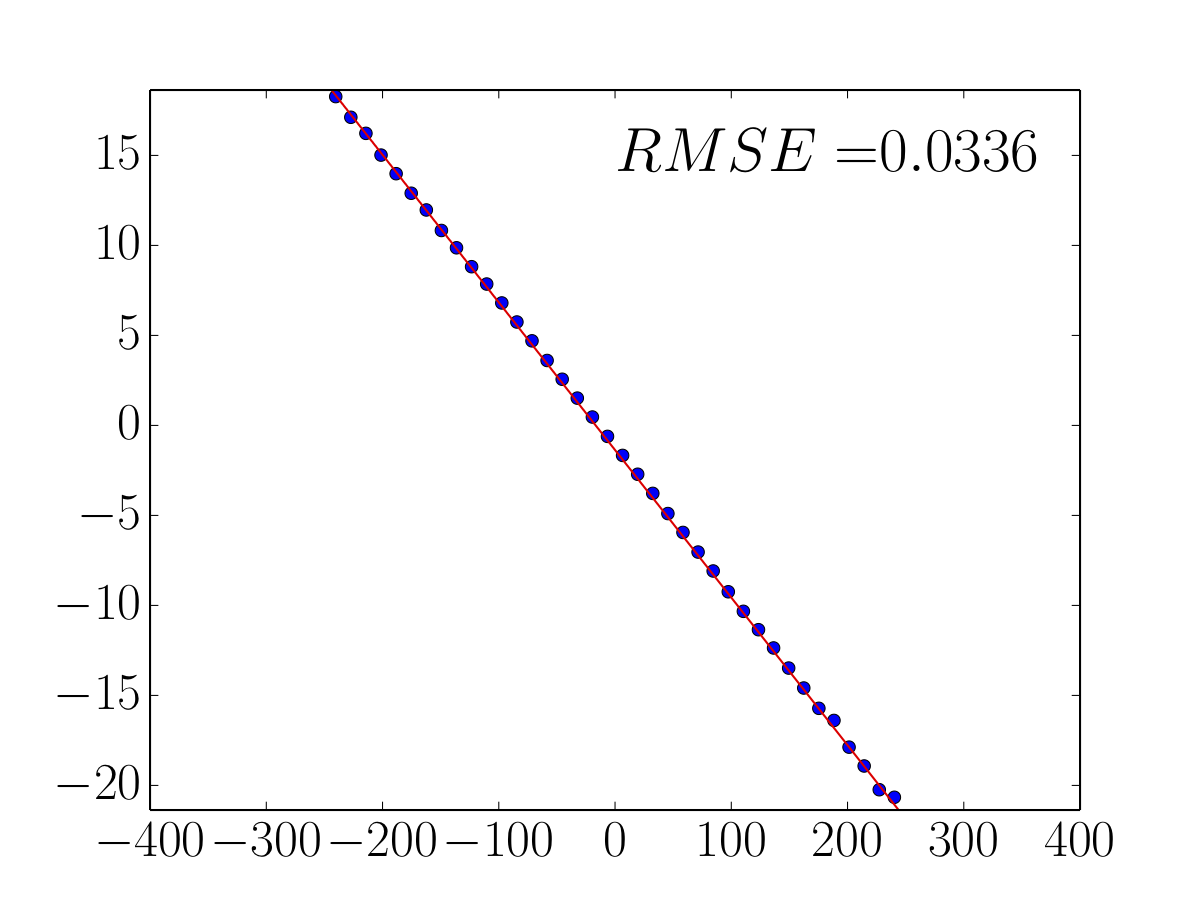
\includegraphics[width=75mm]{figs/B1.png} \\
	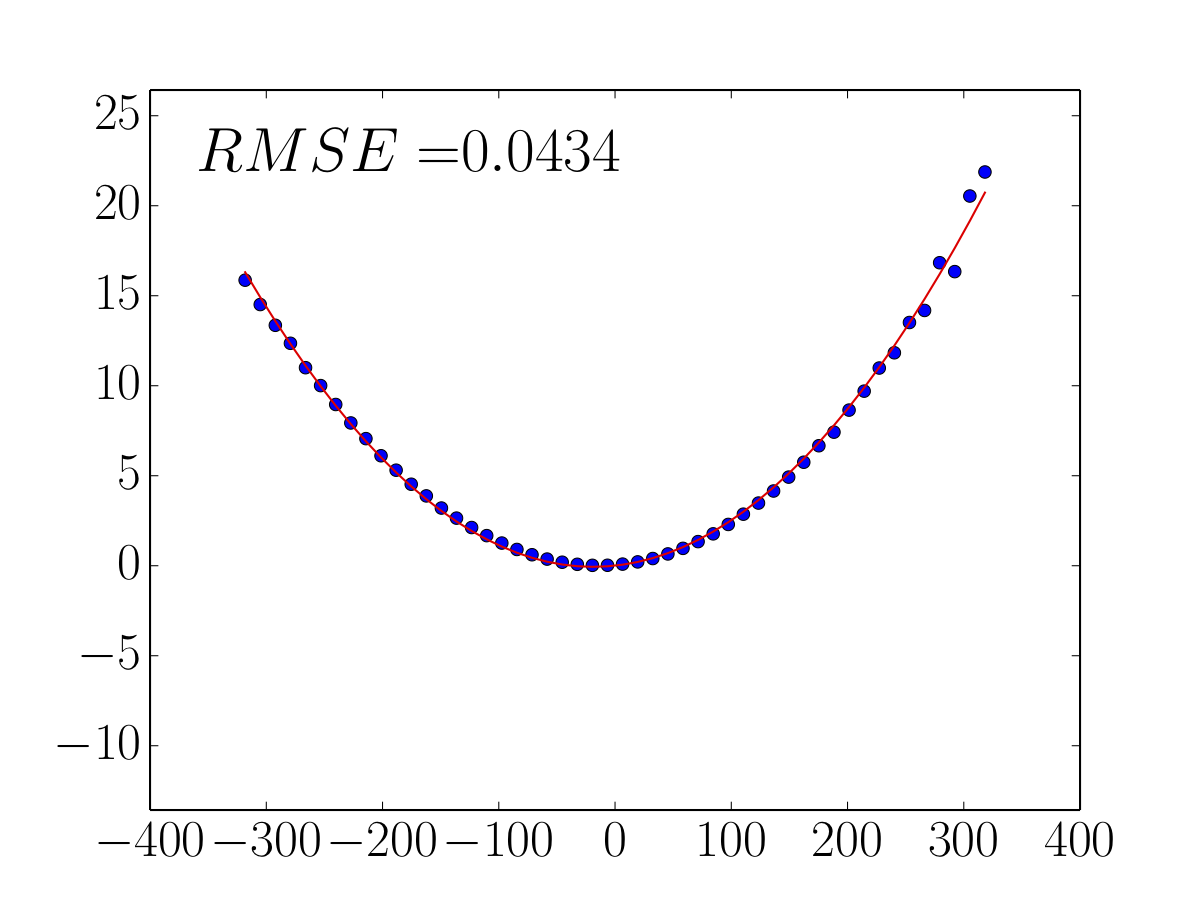
\includegraphics[width=75mm]{figs/B2.png} \\
	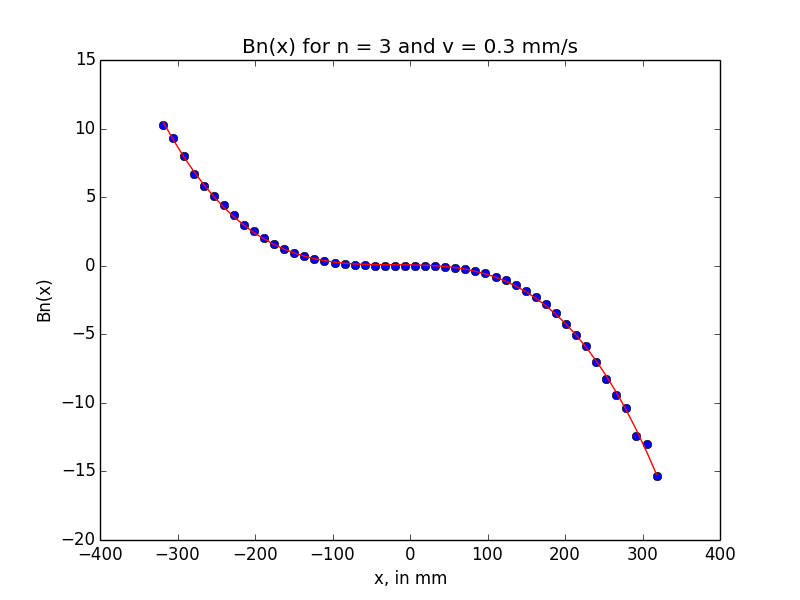
\includegraphics[width=75mm]{figs/B3.png} 
	\end{tabular}
	\caption{From top to bottom, functions $x' \mapsto \Bnv(x')$ for $n = 0,1,2,3$ respectively. Blue points are the actual data, while red lines are the best polynomial approximations. RMSE stands for root mean square error. The $x$-axis are expressed in millimeters.\label{fig:Bnx}}
\end{figure}

With this velocity $\bv = (0.3,0)$ assumed to be unknown, we performed the minimization of the cost function $\mathcal{J}(v)$ defined in~(\ref{eq:Jv}), with a polynomial degree of $n = 2$. For this purpose, we used Powell's conjugate direction method~\cite{powell1964efficient}, which does not require differentiation of the cost function.

We studied the influence of the time during which the object was translating, \ie the angle $\alpha$ of the arc traced by the source $s(t)$ when the object was translating. As an example, for the sinogram depicted in Figure~\ref{fig:sinogram} we have $\alpha = 90^{\circ}$. Table~\ref{tab:results} summarizes all the results, where $\hat{v}$ stands for the estimated value for the velocity $v_1$. We observe that there is a limit below which the accuracy decreased dramatically.

\begin{table}[!ht]
\caption{Results of optimization \label{tab:results}}
\centering
	\begin{tabular}{ccc}
	% $\alpha$ & $95$ & $90$ & $85$ & $84$ & $83$ & $82$ & $81$ & $80$ & $75$ \\
	% \hline 
	% $\hat{v}$ & $0.300$ & $0.300$ & $0.300$ & $0.300$ & $0.300$ & $0.376$ & $0.415$ & $0.436$ & $0.436$ \\
	% \hline
	  $\alpha$ & $\hat{v}$ & $\Vert v_1 - \hat{v}\Vert$ \\
	  \hline
		$95$ & $0.30$0 & $5.55 \cdot 10^{-17}$ \\
		$90$ & $0.300$ & $1.11 \cdot 10^{-16}$ \\
		$85$ & $0.300$ & $1.11 \cdot 10^{-16}$ \\
		$84$ & $0.300$ & $0$ \\
		$83$ & $0.300$ & $0$ \\
		$82$ & $0.376$ & $7.60 \cdot 10^{-2}$ \\
		$81$ & $0.415$ & $0.115$ \\
		$80$ & $0.436$ & $0.136$ \\
		$75$ & $0.436$ & $0.136$
\end{tabular}
\end{table}


\section{Conclusion}
In this work, we have proposed a way to recover the velocity parameters of a translating object in fan-beam CT from a set of projections restricted to an arc of the circular trajectory. The method uses data consistency conditions (DCCs), adapted from~\cite{clackdoyle2015consistency}. Setting the origin of the reference frame at the center of mass of the object, we are in fact dealing with DCCs in the case of an arc of a cycloid. Numerical examples show that these conditions work well in the case of an object translating in a direction which is parallel to the $x$-axis. Further work is in progress to recover the same results for a general translation.


\bibliographystyle{plain}
\bibliography{DCC_translation}


\end{document}

